\documentclass[superscriptaddress,onecolumn,floatfix]{revtex4-2}

\usepackage{graphicx}
\usepackage{epsfig}
\usepackage{color}
\usepackage{amssymb}
\usepackage{amsmath}
\usepackage{array}
\usepackage[loose]{units}
\usepackage[english]{babel}
\usepackage[unicode]{hyperref}
\usepackage{cleveref}
\usepackage{braket}
\usepackage[caption=false]{subfig}
\usepackage{letltxmacro}

\pdfcompresslevel=9

\LetLtxMacro{\ORIGselectlanguage}{\selectlanguage}
\makeatletter
\DeclareRobustCommand{\selectlanguage}[1]{%
    \@ifundefined{alias@\string#1}
      {\ORIGselectlanguage{#1}}
      {\begingroup\edef\x{\endgroup
         \noexpand\ORIGselectlanguage{\@nameuse{alias@#1}}}\x}%
}
\newcommand{\definelanguagealias}[2]{%
  \@namedef{alias@#1}{#2}%
}
\makeatother

\definelanguagealias{en}{english}


\begin{document}
                            
\begin{abstract}
This guide walks you through the steps needed to install the head unit preconditioning kit in your 2023-2025 Ioniq 6. 
\begin{description}
  \item[Step 1: Disconnect 12V] 
  \item[Step 2: Trim]
  \item[Step 3: Harness Connection] 
  \item[Step 4: OBD Mount] 
  \item[Step 4.5: WiCAN Plug-In] 
\end{description}
\end{abstract}
\title{Preconditioning kit install guide: Ioniq 6}
\author{Ioniq Guy}
\author{Electroniq Buttons Boutique}
\email{support@electroniqbuttons.com}
% \affiliation{\GOE}
% \author{Benjamin J. McMorran}
% \email{mcmorran@uoregon.edu}
% \affiliation{\UO}
\date{\today}

\maketitle

\begin{figure}[h]
  \subfloat[]{\label{subfig:overview:harness}
  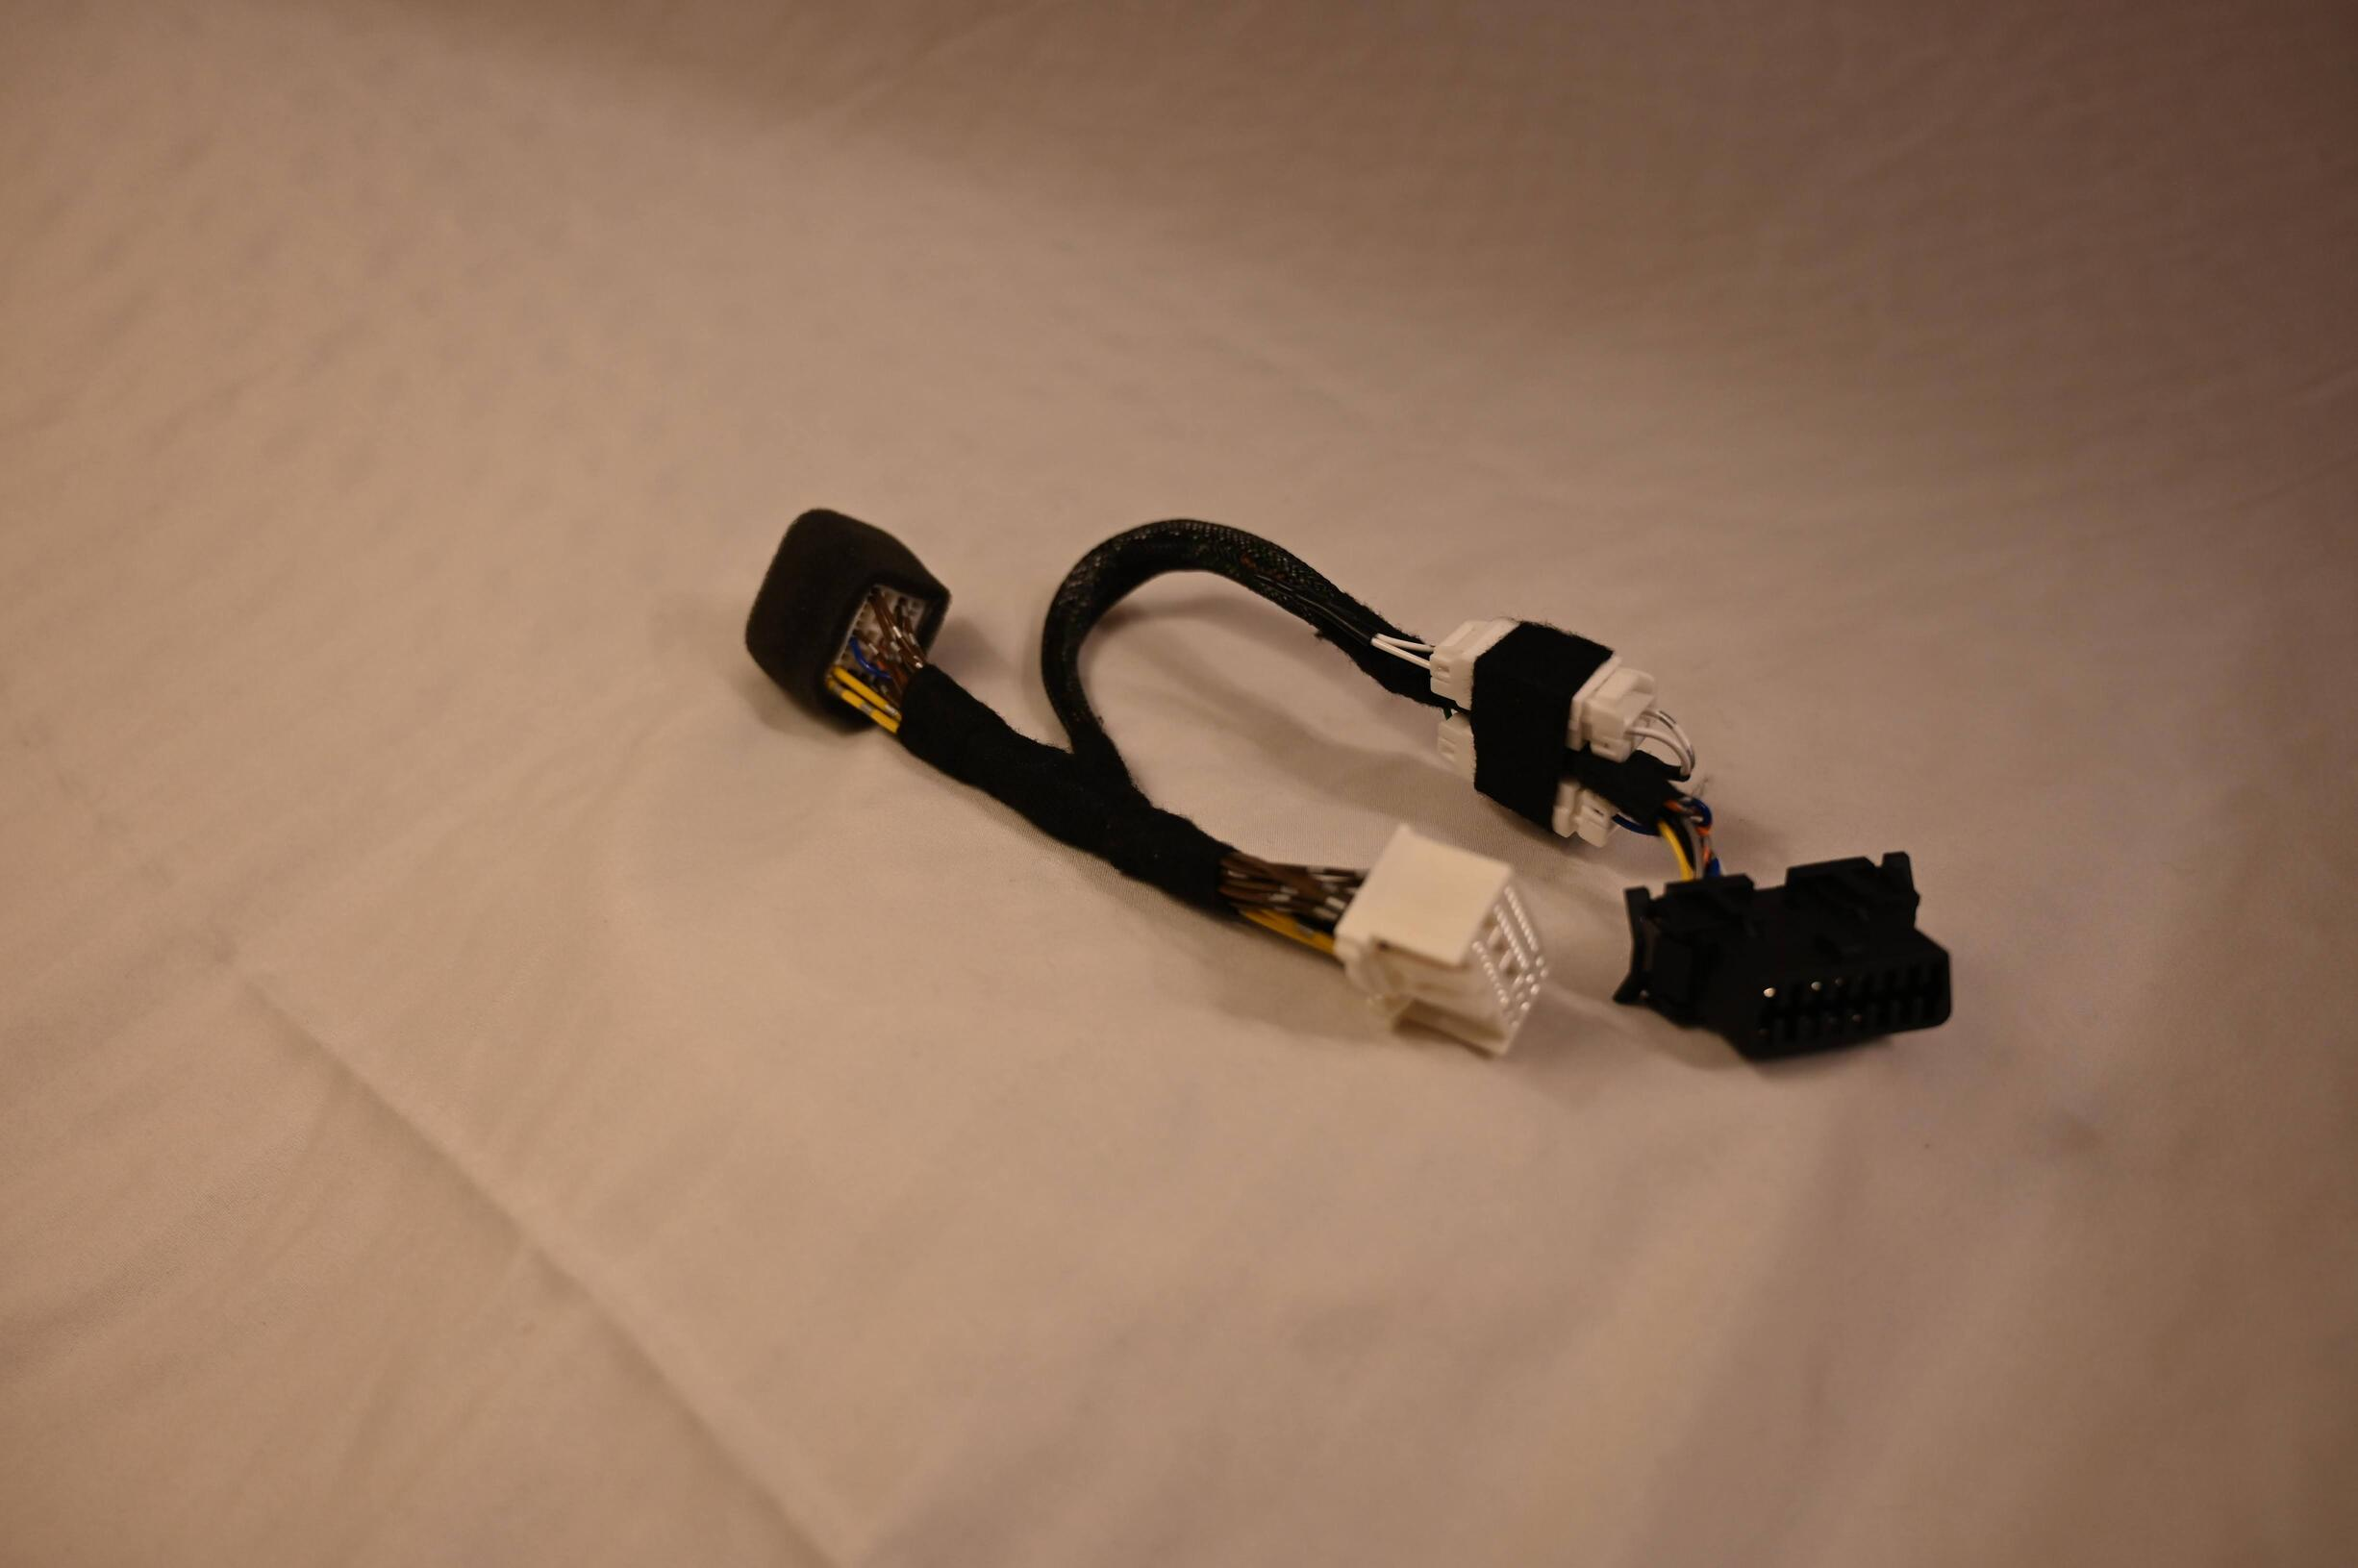
\includegraphics[height=1.95in]{../../../harnesses/head_unit_MITM/photos/whole_harness.jpg} } \\
  % \subfloat[]{\label{subfig:overview:trim}
  % 
\includegraphics[width=6in]{photos/overview_labeled.jpg} }
   \caption{(a) Man-in-the-middle harness. \label{fig:overview}}
\end{figure}

\section{Introduction}
  The purpose of this guide is to illustrate step-by-step instructions for installing the head unit preconditioning kit, or just the head unit man-in-the-middle (MITM) harness, shown in Figure \ref{subfig:overview:harness}. In section \ref{sect:1}, we describe the trim removal process to access the head unit. In section \ref{sect:2}, we describe the process of plugging in the harness. In section \ref{sect:3}, we show attachment of the OBD port and how to plug in the microcontroller. 

Necessary tools:
\begin{enumerate}
  \item 10mm socket or adjustable wrench for 12V battery (not included)
  \item Trim removal tools (included if selected)
\end{enumerate}

Kit components:
\begin{enumerate}
  \item Head unit harness
  \item WiCAN
  \item 70mm OBD mount bracket
  \item 70mm double-sided tape (two pieces included for redundancy)
  \item 4 zip ties
\end{enumerate}
  
\section{Step 1: Remove 12V Negative Terminal} \label{sect:0}
First, always disconnect the 12V battery before removing any electrical connectors! Removing a live electrical connector could cause a discharge and destroy a connector or ECU in your car.

Step-by-step instructions:
\begin{enumerate}
  \item Open hood % (Figure \ref{subfig:12V:hood})
  \item Open frunk  (Figure \ref{subfig:12V:frunk})
  \item Remove panel covering 12V % (Figure \ref{subfig:12V:panel})
  \item Loosen nut on negative side with a 10mm socket % (Figure \ref{subfig:12V:nut})
  \item Remove negative terminal % (Figure \ref{subfig:12V:terminal})
\end{enumerate}

\begin{figure}[h]
  % \subfloat[]{\label{subfig:12V:hood}
  % 
\includegraphics[height=1.5in]{photos/open_hood.jpg} } 
  % \subfloat[]{\label{subfig:12V:panel}
  % 
\includegraphics[height=1.5in]{photos/remove_panel.jpg} }  \\
  % \subfloat[]{\label{subfig:12V:nut}
  % 
\includegraphics[height=1.5in]{photos/loosen_nut.jpg} } 
  % \subfloat[]{\label{subfig:12V:terminal}
  % 
\includegraphics[height=1.5in]{photos/disconnect_terminal.jpg} } 
  \subfloat[]{\label{subfig:12V:frunk}
  \includegraphics[height=1.5in]{photos/frunk.jpg} } 
  \caption{(a) Open frunk. \label{fig:12V}}
   % \caption{(a) Open the hood. (b) Remove panel covering 12V. (c) Loosen nut on negative terminal. (d) Remove negative terminal. \label{fig:12V}}
\end{figure}

\section{Step 2: Trim} \label{sect:1}
The goal here is to get to the treasure chest: the head unit. It's behind a single trim panel called the Crash Pad Under Cover, marked with an X in Figure \ref{fig:step1}.
\begin{figure}[h]
  \subfloat[]{\label{subfig:step1:X}
  \includegraphics[height=2.95in]{photos/x_marks_HU.jpg} } 
   \caption{X marks the head unit. \label{fig:step1}}
\end{figure}

Step-by-step instructions:
\begin{enumerate}
  \item Remove crash crash pad under cover (Figure \ref{subfig:trim:crash_pad_under_cover}): 
    \begin{enumerate}
      \item Use a trim removal tool to gently pry to expose one of the three clips (Figure \ref{subfig:trim:open})
      \item Press on the tab on the clip, indicated by Corbin's thumb in Figure \ref{subfig:trim:open}, to release the clip
    \end{enumerate}
  \item Remove screws holding head unit in place (Figure \ref{subfig:trim:HU_screws})
\end{enumerate}

\begin{figure}[h]
  \subfloat[]{\label{subfig:trim:crash_pad_under_cover}
  \includegraphics[height=1.5in]{photos/harness_installed_1.jpg} } 
  \subfloat[]{\label{subfig:trim:open}
  \includegraphics[height=1.5in]{photos/panel_open.jpg} } 
  \subfloat[]{\label{subfig:trim:HU}
  \includegraphics[height=1.5in]{photos/HU_exposed.jpg} } 
  \subfloat[]{\label{subfig:trim:HU_screws}
  \includegraphics[height=1.5in]{photos/reinstalling_HU.jpg} } 
   \caption{(a) Crash pad under cover. (b) Removing crash pad under cover. (c) Head unit exposed. (d) Removing screws holding head unit in place. \label{fig:trim}}
\end{figure}


\section{Step 3: Harness Connection} \label{sect:2}
This step covers the installation of the harness into the head unit. 

Step-by-step instructions:
\begin{enumerate}
  \item Identify original grey female head unit connector (Figure \ref{subfig:harness:headunit_oe_connectors})
  \item Remove it by squeezing the clip and pulling down 
  \item Insert the female connector you removed into the harness male side (Figure \ref{subfig:harness:harness_male_in})
  \item Insert the harness female side into the head unit (Figure \ref{subfig:harness:harness_in})
\end{enumerate}

\begin{figure}[h]
  \subfloat[]{\label{subfig:harness:female}
  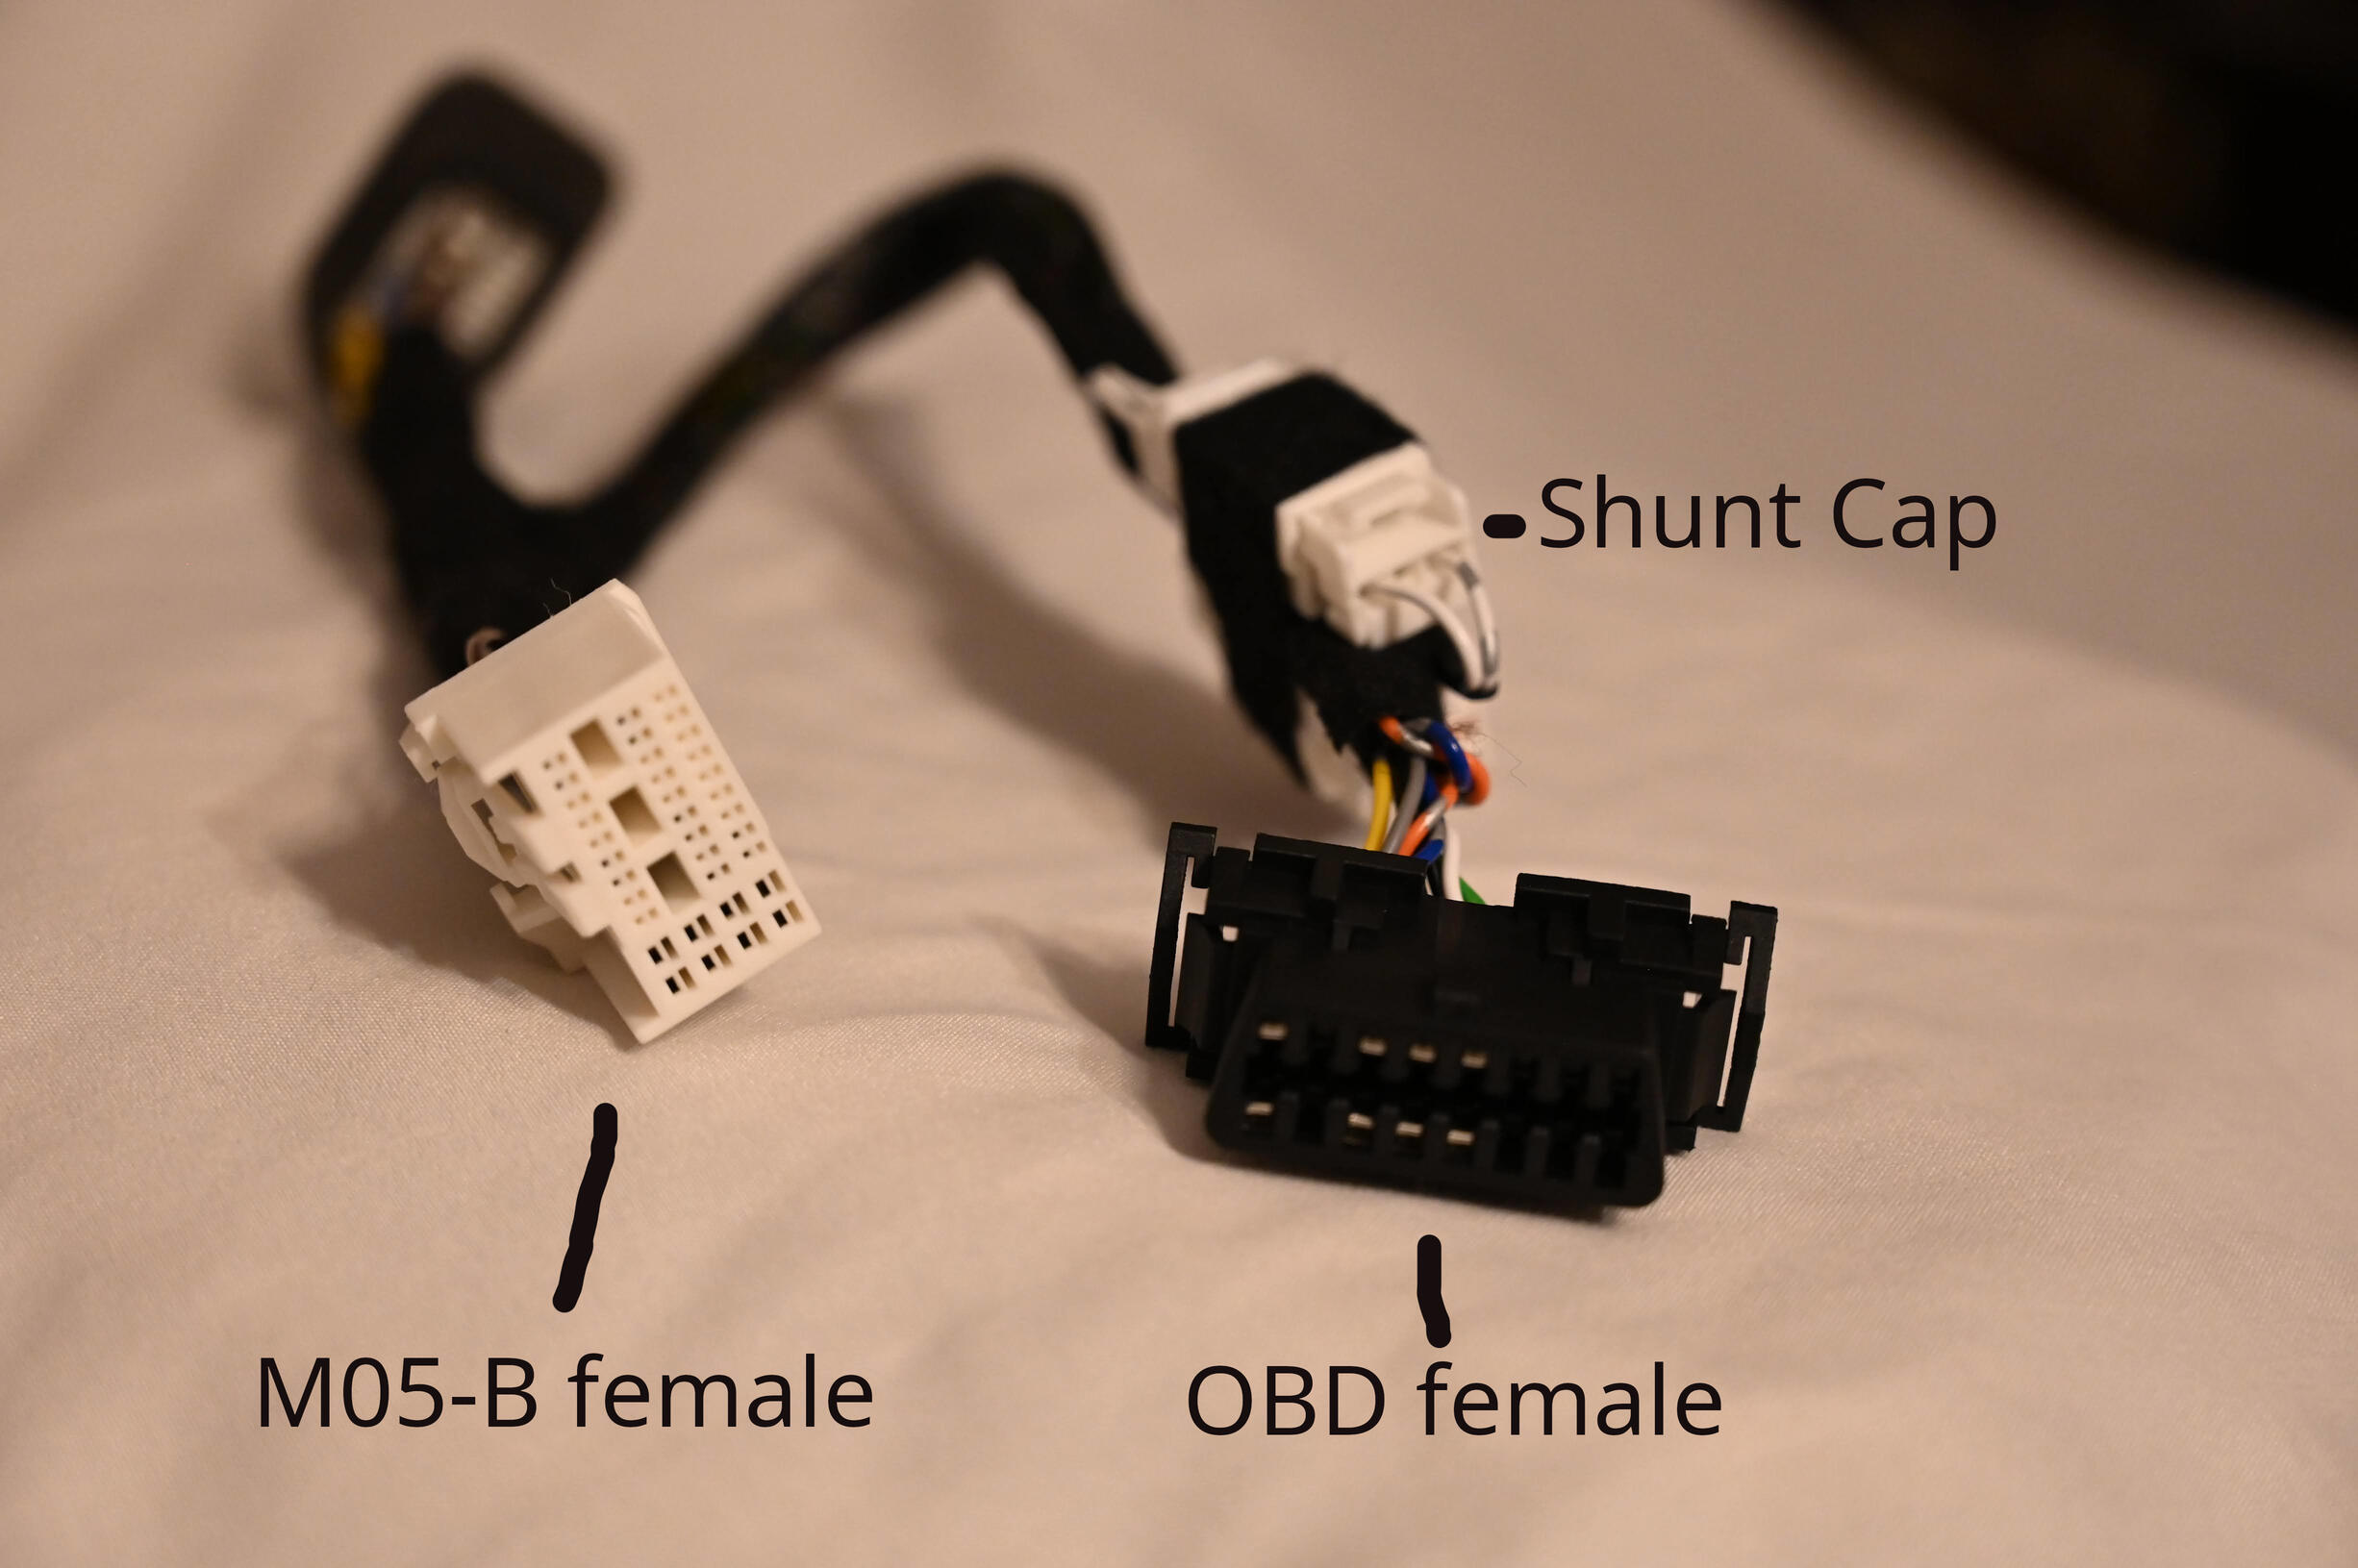
\includegraphics[height=1.5in,angle=0]{../../../harnesses/head_unit_MITM/photos/labeled_connectors_MITM_harness.jpg} } 
  \subfloat[]{\label{subfig:harness:male}
  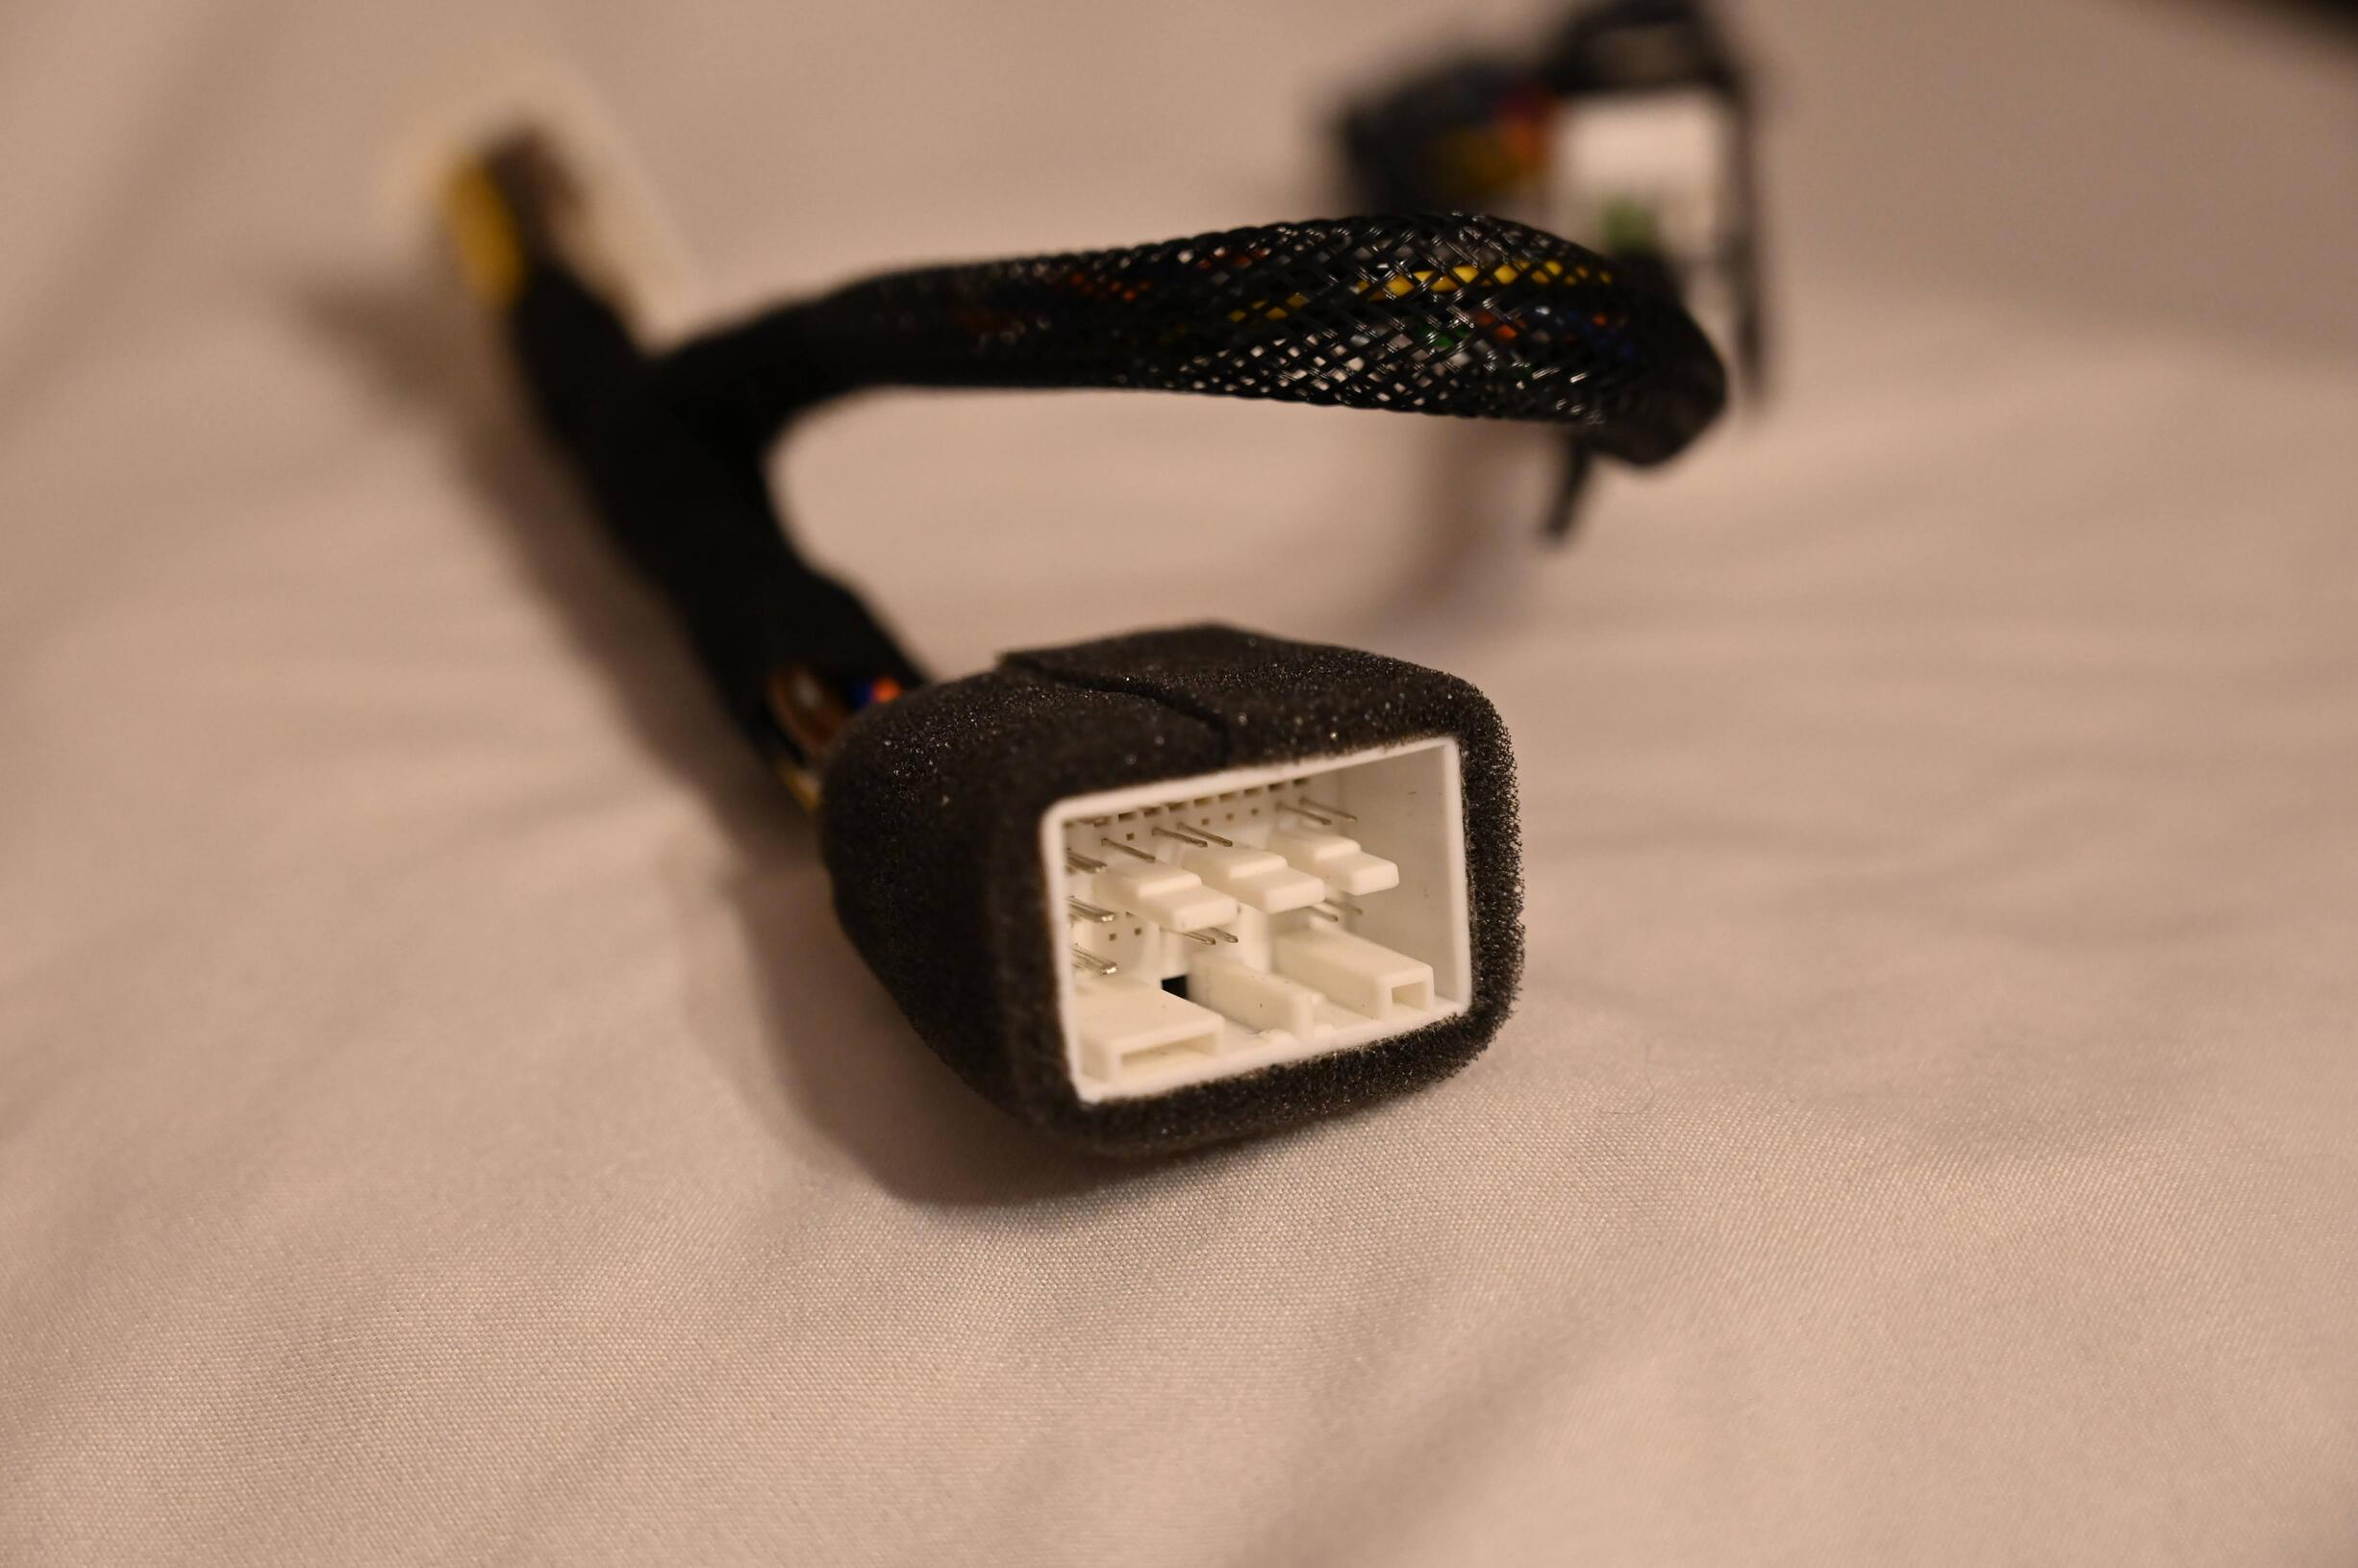
\includegraphics[height=1.5in,angle=0]{../Ioniq5/photos/male_harness_end.jpg} }  \\
  \subfloat[]{\label{subfig:harness:headunit_oe_connectors}
  \includegraphics[height=1.5in,angle=0]{photos/HU_dangling_clip_detached.jpg} } 
  \subfloat[]{\label{subfig:harness:harness_male_in}
  \includegraphics[height=1.5in,angle=0]{photos/harness_installing_3.jpg} } 
  \subfloat[]{\label{subfig:harness:harness_in}
  \includegraphics[height=1.5in,angle=0]{photos/HU_dangling_clip_detached_2.jpg} }  
   \caption{(a) Labeled photo showing female harness connector. (b) Male harness connector. (c) Head unit with original connectors plugged in. (d) Female connector (grey) removed from head unit. (e) Harness installed in head unit. \label{fig:harness}}
\end{figure}
\section{Step 4: OBD Mount} \label{sect:3}
In this step, we mount the OBD end of the harness securely and plug in the WiCAN. 

Step-by-step instructions:
\begin{enumerate}
  \item Thread OBD end over head unit mount bracket (Figure \ref{subfig:obd:thread_obd})
  \item Re-mount head unit. (Figure \ref{subfig:trim:HU_screws})
  \item Plug OBD female into provided bracket, if not already mounted
  \item Use double-sided tape to mount bracket to a flat trim surface
  \item Use zip ties to attach harness to other wires and mount points 
  \item While holding bracket, plug in WiCAN (Figure \ref{subfig:obd:wican})
\end{enumerate}

\begin{figure}[h]
  \subfloat[]{\label{subfig:obd:thread_obd}
  \includegraphics[height=1.5in,angle=0]{photos/harness_installed_HU_detached.jpg} }  
  \subfloat[]{\label{subfig:obd:installed}
  \includegraphics[height=1.5in,angle=0]{photos/harness_installed_1.jpg} } 
  \subfloat[]{\label{subfig:obd:wican}
  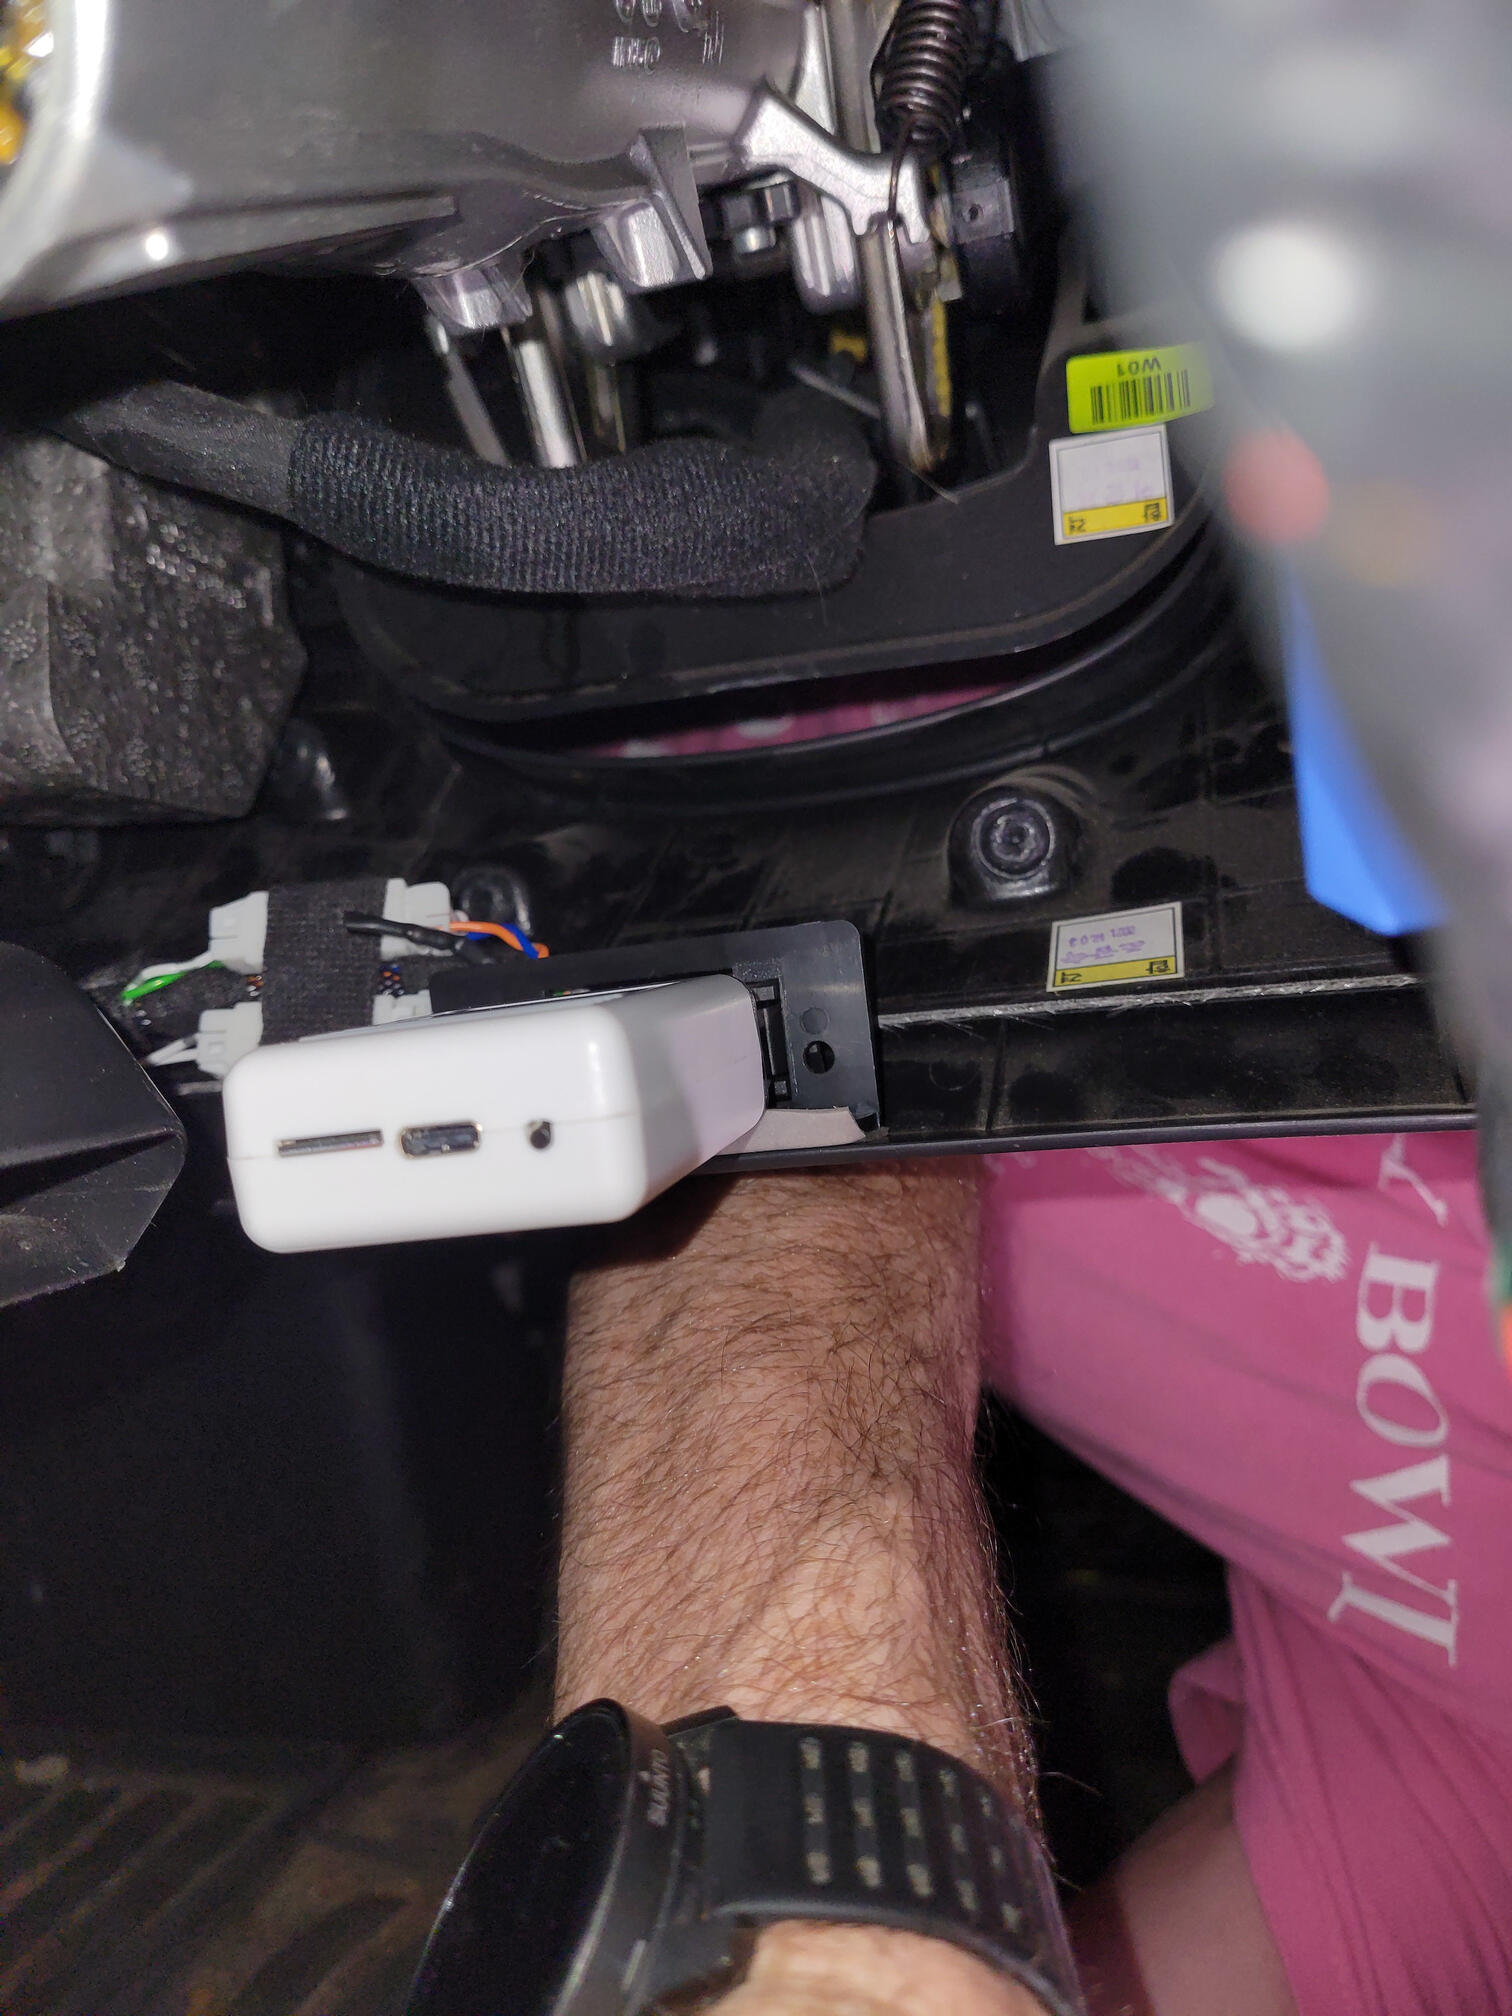
\includegraphics[height=1.5in,angle=0]{../Ioniq5/photos/wican_inserted.jpg} } 
   \caption{(a) OBD threaded over head unit mount bracket. (b) Harness zip-tied to existing wire. (c) WiCAN inserted into OBD. \label{fig:obd}}
\end{figure}

\section{Step 5: Clean up} \label{sect:4}
Reverse the trim removal steps. Make sure trim clips are aligned, and then firmly pop the trim panels back into place. Reconnect 12V battery negative terminal. The WiCAN should immediately show a blue light. Change your WiCAN password: \href{https://meatpihq.github.io/wican-fw/config/wifi}{https://meatpihq.github.io/wican-fw/config/wifi}. You can connect you your WiCAN directly by finding a WiFi network named 'WiCAN\_xxxxxxx' and going to \href{http://192.168.80.1/}{http://192.168.80.1/} in your browser.
% \appendix 
\end{document}